% This file (thesis-main.tex) is the main file for a master's thesis.
\documentclass {udthesis}
% preamble

% Include graphicx package for the example image used
% Use LaTeX->PDF if including graphics such as .jpg, .png or .pdf.
% Use LaTeX->PS->PDF if including graphics such as .ps or .eps
% Best practice to not specify the file extension for included images,
% so when LaTeX is building it will look for the appropriate image type.
\usepackage{graphicx}
\graphicspath{{./images}}
\usepackage[section]{placeins}
\usepackage{caption}
\usepackage{subcaption}
                
\begin{document}
% 
% This is the Title and Approval Page file (thesis-tap.tex) for
% a master's thesis.
%
% The order of the commands below is very important.
% You may choose to add or eliminate a \prefacesection 
% in the front material but the order should remain 
% the same especially \maketocloflot followed by 
% \prefacesectiontoc{Abstract}

% Title and author are also used for PDF file properties
% No special character or commands can be used for the PDF definition; 
% use the [options] paramater to specify a different title or author 
% to remove special characters or commands like \\ for example.
\title[Designing a Modular Testing Platform for Digital-to-Analog Signals]{Designing a Modular Testing Platform for Digital-to-Analog Signals}
\author{Alex Chacko}
\type{thesis}
\degree{Master of Science}
\majorfieldtrue\majorfield{Major}
\degreedate{Semester Year}
% Optional PDF properties
\keywords{Keyord,Keyword,Keyword}
\subject{Subject}

\maketitlepage % Generates Title Page

\begin{approvalpage}
	\chair{Xxxx Xxxx, Highest Degree}{Chair of the Department of Xxxx}
	\dean{Xxxx Xxxx, Highest Degree}{Dean of the College of Xxxx}
	\dean{Xxxx Xxxx, Highest Degree}{Dean of the College of Xxxx}
\end{approvalpage}

\begin{front} % Starts front material (Roman style page numbers)

	\prefacesection{Acknowledgments}
	%I would like to thank my parents Thomas and Ambika, my sister Christy, and my cat Freya for their unwavering support and love throughout my school and research career. \par
I would also like to thank the team at CDS and CVORG. My advisor Dr. Fouad Kiamilev offered me access to a practical research opportunity as an undergraduate I could never have hoped to receive elsewhere. This project has given me new perspectives on engineering and collective leadership. \par
My teammates and coworkers have cultivated a warm and encouraging research environment. We are all working towards common objectives and are never discouraged from asking questions and experimenting. The entire CVORG and CDS community made honing in on my specific interests a natural process. I would, however, like to specifially like to thank my fellow graduate and undergraduate researchers Hagan Beatson, Michael Richards, Mike Joyce and Matt Greenlee for their dedication, shared curiosity, and collaborative natures during our work together. Former and present senior group members and employees including Alexis Deputy, Jaclyn Singh, Tianne Lassitter, Miguel Hernandez, Tyler Browning, Aaron Landwehr, Chris Jackson and Daniel May have also offered invaluable help and guidance throughout my time in the group. Thank you all so much. % This file (acknowl.tex) contains the text
	% for the acknowledgments or type text here.


	% Table of Contents is always created, but you
	% may set \tablespagefalse and \figurespagefalse 
	% if you don't want these generated automatically
	% (i.e. List of Tables and List of Figures).
	% These are set to true by default (i.e. \tablespagetrue,
	% \figurespagetrue).

	% Uncomment if you do not want a List of Figures.
	%\figurespagefalse

	% Uncomment if you do not want a List of Tables.
	%\tablespagefalse 

	\maketocloflot

	\prefacesectiontoc{Abstract}
	%The Infrared Scene Projector (IRSP) market has developed to require high resolution, frame rates, and dynamic range for projected videos. Within the IRSP, Infrared LEDs (IRLEDS) are driven by analog signals from a control circuit. These LEDS require precise output levels and consequently the system utilizes hardware-in-the-loop monitoring of output. The analog subsystem of our IRSP demands high integrity and hardware capabilities to avoid bottlenecks and deliver clean signals. This paper describes a newly designed testing procedure for the IRSP's current analog system, as well as the lessons learned from this process used towards designing the analog component of our next generation IRSP. % This file (abstract.tex) contains the text
	% for an abstract or type text here.

\end{front}


                   % This file (thesis-tap.tex) contains the Title
                   % and Approval Page information for a master's thesis.

%
% This is Chapter 1 file (chap1.tex)
%
\chapter{Introduction}

\section{SLEDs Background}

Infrared imaging and detection is used in various industries and services around the world. Since infrared light exists outside the human-visible light spectrum, it requires specialized hardware and testing procedures to ensure proper performance. Infrared applications generally require high speed and precision, which means that testing infrared systems is a vital step in ensuring their success. \par
A system must be "statically" and "dynamically" calibrated with an accurate infrared source. A static calibration only requires scientific test equipment to measure radiance. Dynamic calibration is much more involved and requires a throrough understanding of the system in question. To dynamically test, the system is placed under more realistic and changing conditions, such as having to react appropriately to moving objects or images. A common solution for this need is the Infrared Scene Projector (IRSP) which can be used to project infrared images and video to test a desired device. \par
IRSPs display realtime IR scenes that simulate true IR signals for their targets. Since infrared depends on physical information (temperature), simulating this as a signal requires specialized hardware. This hardware is used to turn commands from the users into analog display signals as well as read feedback from the display device and adjust its own parameters accordingly. This "hardware-in-the-loop" approach can allow a system to accomodate for various physical effects or issues within the display. Since infrared displays are analog devices, they cannot be precisely analyzed without some sort of readback and processing to view output. A typical system design is shown below. \par
\begin{figure}[!htb]
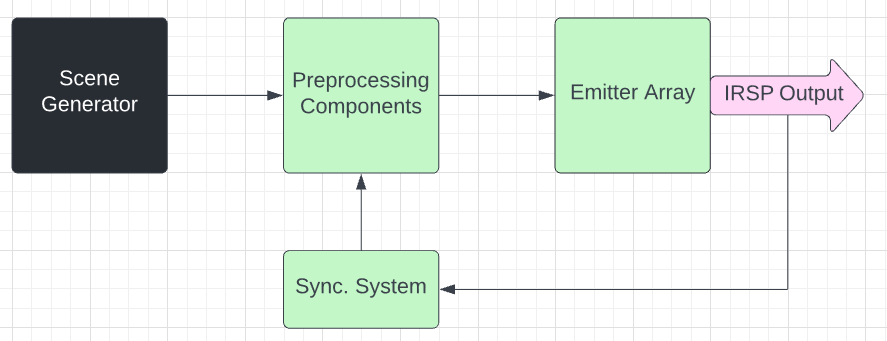
\includegraphics[width=10cm]{irsp_block_diagram}
\centering
\caption{General IRSP architecture}
\centering
\end{figure}
Testing is one of the most important aspects of any system design, as it is the bottleneck for how many reliable systems can be built \& validated. This work consists of a new approach to manually test the high-speed analog amplifier circuits within the system, as well as considerations \& redesigns for the next generation of these devices. 

\section {Motivation}
IRSPs can be characterized by multiple factors, of which two of the most important are frame rate and output temperature range. Frame rate can be described as the number of discrete outputs from the display device per second. The frame rate is directly tied to the rise time of individual pixels, which is fully dependent on the display architecture and physical properties. The temperature range represents different "colors" or ranges of IR light that the projector can display. An ideal device has both high refresh rate and high max temperature to overcome the challenges of temperature-based projection. \cite{marks} \par
Much of the IRSP market is dominated by resistor array devices. By heating up resistors (mapped to each pixel) to specific points with controlled current input, the device can simulate temperature output for an infrared image. The use of resistors limits the benefits of this approach, however. \cite{spie:2015} Resistor arrays depend on raising temperatures to the actual desired temperature of the projected image. While innovative, resistors cannot dissipate heat quickly, limiting their rise time. The characteristics of the resistors are a hard limit on refresh rate, forcing most designs to stay under 500Hz. Additionally, higher projected temperatures will further increase the rise time, since the resistors will have to physically cool down from this temperature level. By limiting the max temperature output, designers can ensure that pixel rise time will consistently stay within a certain range. \par
Since 2008, CVORG has been at the forefront of developing an Infrared LED-based IRSP with a full suite of custom hardware and software control. \cite{peyman} The success of the current iteration of the system has allowed us to continue researching improvements and changes to the system that would further expand on the technology's potential. Our technology is now targeting a 1024 x 1024 display at 2KHz. \par
After successfully developing the technology to a certain point, it was considered stable enough to reproduce and iterate on. The process of building and testing each component of the system provides one with an intimate knowledge of the functions and requirements of individual hardware components, as well as limitations to be targeted later. \par
One of the most important links in the system's chain consists of the digital-to-analog conversion and subsequent amplification. These amplified analog signals are used to drive the display, making their functionality and speed a top priority. \cite{tianne} As such, it was imperative to create reliable testing procedures for such components. The relevant systems, components \& design methodology for this portion of the system will be described in detail below. \par
    % This file (chap1.tex) contains the text
                   % for Chapter 1.
                   
%
% This is Chapter 2 file (chap2.tex)
%
\chapter{System Overview}
Using a combination of digital commands and analog signals users can precisely command and utilize the display at the high frequencies required by the application. The system has been developed over the years to be user-friendly and configurable for many different applications. The associated technologies will be briefly explored below.
\begin {figure}[h]
\includegraphics*[width=10cm]{system_overview}
\centering
\caption {SLEDS IRSP Overview \cite{chris}}
\centering
\end {figure}


\section{SLEDS Array}
As mentioned before, infrared projection requires high-speed analog signals and full user control. The LED array itself is hybridized to a Read-In Integrated Circuit (RIIC), a 10V chip which is digitally instructed by a close-support unit. This hybridized unit in its temperature-controlled enclosure is referred to as the Dewar. The first iteration of this LED array named SLED (Superlattice Light-Emitting Diode System) was constructed in 2008 with a resolution of 68 x 68 pixels. In this early stage, no driver had yet been developed to control the RIIC. \cite{chris}\par
To drive such a complex analog device, specialized electronics and communication are required to turn human commands into infrared signals. The first drive system for the SLED array was developed in 2011 and helped lay the groundwork for the next iteration of SLEDS, consisting of a 512x512 display and 48 micrometer pitch size.\cite{chris} \par
Further versions of SLEDS were created over the years to fulfill different requirements. TCSA (Two-Color SLEDS Array) was developed in 2016 and capable of driving the LEDs at two separate wavelength bands. NSLEDS (N3 Superlattice LED System) was also developed around this time. This array was capable of driving a 1024x1024 display for the first time. The next advancement, HDILED (High-Definition Infrared LED) was the first 2048x2048 display in the world when it was finished. \par
\begin {figure}[h]
\includegraphics*[width=10cm]{timeline1}
\centering
\caption {SLEDS Timeline \cite{chris}}
\centering
\end {figure}
\begin {figure}[h]
\includegraphics*[width=10cm]{timeline2}
\centering
\caption {SLEDS Timeline, Part 2 \cite{chris}}
\centering
\end {figure}

\section{RIIC Overview}
The RIIC is a 10 volt IC that is hybridized with an array of IRLEDs to directly drive them using CMOS logic. A dual-circuit system allows the array to display at different dynamic ranges, a "weak gear" and "strong gear".
\begin {figure} [h]
\includegraphics*[width = 8cm]{riic_cmos}
\centering
\caption {Single Pixel RIIC Schematic \cite{miguel}}
\centering
\end {figure}
Each pixel is driven by a strong/weak pair of NMOS transistors, which do not take up as much space as PMOS and allow for greater resolution as a result. \par
The RIIC is divided into four quadrants that can be individually commanded. Due to the nature of the driver firmware that will be discussed later below, this quadrant approach allows great control over the display. \cite{miguel} Each quadrant has 2-32 input channels depending on the desired configuration. Configuration is performed using an SPI register on the RIIC, shifting in data when commands are received. \par

\section{CSE Overview}
The RIIC/LED hybrid is driven by a close-support electronics system, or CSE. While the CSE was a response to the need for a RIIC driver, it is also the culmination of many years of work and development. The system architecture consists of an FPGA, DACs, Amps, and I/O boards. This array of hardware completes the loop from a user on any PC to the IRLED array, making the projector a viable product. This hardware has been redesigned and iterated on for years, and is now being fully upgraded to a second revision consisting of smaller components and more efficient signal integrity strategies.

\section{Scene Generation and NUCPC}
The final ingredient necessary in the IRSP chain is the Scene Generator. While scene generation technology is far beyond the scope of my work, a general overview is necessary to understand the system. A scene generator is to the projector what a media player is to a television. Most of these scene generators are proprietary black boxes, documented by the creators to be sold to end users \cite{chris} Scene generators can communicate over nearly any physical interface, but the standards must be agreed upon between the manufacturer and user. A common display protocol is DVI, as it is fairly well documented and easy to understand. HDMI is another possible choice, but it is a more complex and less openly documented standard. \par
To generate a scene, a GPU is usually necessary to create images and transmit them over the chosen display protocol. The generator will use frames created on the GPU to send over to the IRSP. The next step is called "Non-Uniformity Correction," which is the process of analyzing predetermined output from the IRSP to determine radiance properties of each pixel. Pixel data is placed into a table used by the scene projector and used to accomodate for irregularities in the LEDs. These irregularites are nonlinear which is why they require analysis and writeback rather than simple algorithmic correction. Once the NUC process is complete, the desired images can be projected onto the display device. \par
\begin{figure}[!htb]
	\includegraphics*[width=15cm]{scene_gen_example}
	\centering
	\caption{Example scene generator in IR system \cite{chris}}
	\centering
\end{figure}
Since our research group did not have access to a proprietary scene generator, they developed a pseudo-scene projector using what was dubbed a Non-Uniformity Correction PC (NUCPC). This NUCPC is connected to the CSE through HDMI, and image data is generated by an Nvidia graphics card\cite{chris}.    % This file (chap2.tex) contains the text
                   % for Chapter 2.
%
% Chapter 3
%
\chapter{PDP vs. Conventional Display Protocols}
\section{DVI \& HDMI}
Early scene generators used the DVI protocol, which is a simple and well understood standard. Unfortunately, they are also quite large connectors that did not fit well into the CSE design. For this reason, HDMI was chosen as the display protocol for NUCPC to CSE. HDMI uses the same electrical levels as DVI which kept it compatible with preexisting scene generator technology. \par
While they are good solutions, these display protocols are also rather limited. They are forced to remain compatible with even older protocols such as VGA. An example of typical display function is shown below. Video data is sent in sequential horizontal lines. Once the boundary of the display is reached, a "blanking period" is entered to reset the device's row/frame. The blanking period is recognized by a sync signal, which means that bandwidth is required for non-video data. If blanking periods were able to be reduced, it would inversely increase the potential frame rate. \par
Fixed frame-rate display protocols are also inherently limited. If a new frame is not necessary, the last frame will be retransmitted. Bandwidth is static which is useful for the reliability of consumer products, but less useful for a high-speed infrared projector. As such, utilizing the potential bandwidth of HDMI became a top priority and the foundation for the CSE firmware. 
\begin{figure}[h]
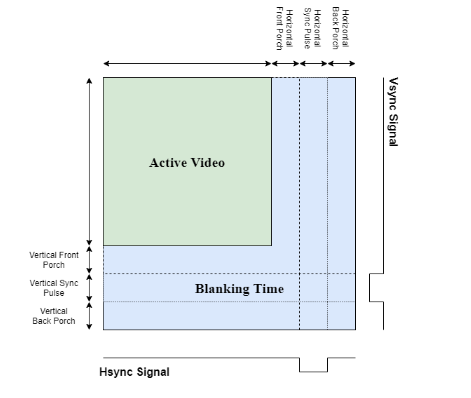
\includegraphics[width=10cm]{display_protocol}
\centering
\caption{An example of timing in display protocols}
\centering
\end{figure}
\section{PDP}
The Packetized Display Protocol (PDP) is the communication protocol for the CSE to LED array. The initial vision for PDP consisted of a "physical layer agnostic method of pixel data transmission capable of providing and addressing latency guarantees while maximizing bandwidth utilization" \cite{pdp_ieee}. Unlike traditional display communication protocols, PDP does not operate on entire display frames, and instead splits any projected scene into regions known as sub-frames. These sub-frames can be written to individually, greatly increasing bandwidth utilization and allowing for high frame rates beyond any traditional HDMI connection. \par
Sub-frames are marked by the PDP firmware with packets denoting their x and y coordinates. PDP communication packets will then consist of a packet header for draw location followed by the desired data. This divide-and-conquer strategy allows the NUCPC to only send frames when they require updates and therefore update relevant subframes at much higher frame rates than normally possible \cite{chris}. IRSP is an incredible application for this concept, as many scenes only have small regions that require updates. An example scene may contain a subframe changing at 200Hz, another at 50Hz, and yet another remaining static. Over a traditional display protocol, displaying any of these regions at the appropriate rates would be impossible due to the entire frames being sent at preset intervals. PDP, however, allows the NUCPC to utilize far more HDMI bandwidth to only send packets relevant to the subframes.\par
\begin{figure}[h]
	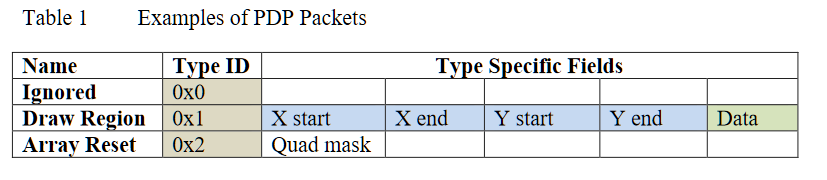
\includegraphics[width=10cm]{pdp_table.png}
	\centering
	\caption{Brief example of PDP Packet}
	\centering
\end{figure}
PDP can be used in two modes. The method of splitting and refreshing subframes is known as "streaming mode". Users may also opt to use it in a typical display mode where the entire frame is sent at a fixed refresh rate. This is known as "backwards compatibility mode". While there is nothing innovative about this mode, it is necessary to maintain compatibility with existing scene generation technology.\par
\begin{figure}[h]
	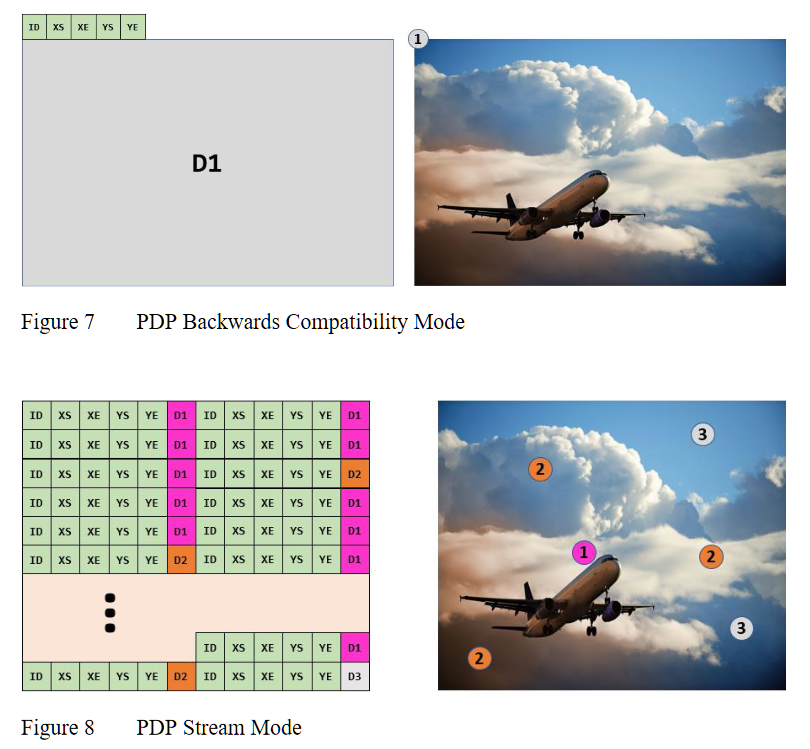
\includegraphics[width=10cm]{pdp_backwards_compatibility}
	\centering
	\caption{Example of packet organization in each mode}
	\centering
\end{figure}
PDP was previously described as being "physical layer agnostic" \cite{pdp_ieee}. The protocol can theoretically be implemented over any physical medium such as DVI or ethernet. The initial implementation utilized HDMI to maintain compatiblity with existing technology, but a future revision is moving the physical medium to SFP+. Improvements to the CSE hardware will be briefly discussed in a later section.
%
%Chapter 4
%
\chapter{CSE Architecture}
\section{CSE Hardware Overview}
The CSE is comprised of two gigabit-speed input cards, a mainboard powered by an FPGA, eight DACs connected to the FPGA, eight amplifier cards (one for each DAC) and a pair of interface boards \cite{chris}. The input interface cards have HDMI I/O ports and connect to the NUCPC or external scene generator to receive input. Each interface card is connected to the main FPGA via FPGA Mezzanine Card (FMC) slots. The FPGA is host to a MicroBlaze soft processor and uses its eight remaining FMC slots for DACs. Each DAC outputs to an amplifier card, creating the analog driving inputs for the RIIC. All amplified signals are routed out through the interface board to be connected to the RIIC through ribbon cables. 
\section{Datapath}
Once the scene generator provides video input, the HDMI cards decode and send the video stream to the FPGA. Since the FPGA uses a soft processor, it can be interfaced with in C to control registers \cite{chris}. The processed data is then distributed amongst the eight DAC slots in accordance with the packets defined by PDP. Each DAC card holds two dual-channel DAC components for a total of 32 channels. Once the digital input has been converted to analog, the amplifier cards boost the output and send it through the interface boards. Each interface board has power input from a PSU and power output for the DACs and Amps, and also contain boost components to convert the 2.5V amplified output to 5V for the RIIC to read. \par
\begin{figure}[!htb]
	\includegraphics*[width = 15cm]{cse_datapath}
	\centering
	\caption{CSE Architecture Overview}
	\centering
\end{figure}
\section{Hardware Revisions \& System Upgrade Plans}
After many years of development, the CSE reached a level of maturity to be considered a cohesive product (internally dubbed Nessie). Due to ever-increasing requirements from customers and breakthroughs in the technology, the group has moved to target a multi-CSE platform capable of each driving a quadrant of an array (now known as Nessie2). By increasing the number of output machines, frame rates can be quadrupled and resolution can be doubled \cite{chris}. To compare, the previous system (CSE + SLEDS) would effectively be one quarter of this entire setup. The main challenge facing the system architecture is proper synchronization, as this is vital to ensure all quadrants are being controlled in the same time domain.\par
Another major change coming to the system architecture is the placement of all analog systems onto the Dewar enclosure rather than inside the CSE. This means the CSE will only handle digital video conversion, and send these values to amplifiers directly on the Dewar. The overall datapath will remain the same with a scene generator interfacing with the FPGA through an SFP+ interface. The FPGA will distribute video data amongst the DACs and then routed outside to the Dewar to be amplified and read. Plans for the Nessie2 amps based on lessons learned from the Nessie1 amps will be discussed later.

%
% Chapter 5
%
\chapter{CSE Analog Components}
\section{Analog Circuit}
In order to develop a better testing procedure for the current amplifier circuits as well as begin development of the next generation, some exploration of the initial designers' writing was required. Analog output from the CSE was addressed to each pixel of the IRSP. Due to the sensitive nature of digital-to-analog communications and the unique load requirements of the system the entire system architecture had to be measured and mapped out. To do so, the system was split into various sections representing gain and load stages. \cite{marks}. The first stage (DAC Buffer) was responsible for terminating the differential output of the DAC and turning it into a single-ended signal. The next stage was the Cable Driver, a gain stage which was responsible for driving interface board communication and ribbon cable signals. This stage provides some, but not all of the voltage gain required to drive the RIIC from 0-5V. The ribbon cables would output to the final stage known as the Dewar Driver. This stage provides the remainder of the gain required to drive the RIIC at 5V. The Dewar output stage was a 10nF load and required a 0-10V swing from the amplifiers. \par
\begin{figure}[!htb]
	\includegraphics*[]{analog_stages}
	\centering
	\caption{High-level schematic of the analog gain \& impedance stages}
	\centering
\end{figure}
\section{Understanding the Requirements}
To properly test, validate and repair the amp cards, one requires an understanding of the card's place in the system. The card was responsible for passing digital-to-analog converted signals with 16-bit resolution at high speeds, and any issues would be directly visible in the projected video. The amp card received inputs from a 16-bit DAC with a 250 Megasamples per second output \cite{marks}. For digital information to be properly decoded as an analog signal, the converter must settle on values at an acceptable speed with negligible margin of error. As bit resolution increases, the margin of error should decrease. Output voltage from the DACs has been previously tested and documented giving us a base for what voltages needed to be swept for validation. \par

\section{Settling Time}
In any digital-to-analog system, designers must account for physical characteristics of electronics. Every DAC has a delay between input and response, known as Delay Time. The DAC then enters a Slewing period, where it tries to approach the target current or voltage output as fast as possible (current level in the case of our specific DAC). As the DAC approaches the target, slope decreases and the DAC oscillates between over- and under-estimates of the value until finally settling on a DC output. While an ideal DAC will settle on a precise output, most DACs will continue to oscillate between values if it is unable to discern their mean, especially in practical situations. The mathematical account of this phenomenon is called the Error Band. \par
\begin{figure}[!htb]
	\includegraphics*[width=15cm]{error_band}
	\centering
	\caption{Example DAC output}
	\centering
\end{figure}
\section{Error Band}
The maximum acceptable error band is notated as
\begin{math}
	\frac{Vout}{2^n}
\end{math}
where Vout represents the maximum voltage output of the device and N represents the desired bit resolution. An 8-bit system with 4V max output, for example, has an error band of
\begin {math}
\frac{4V}{2^8}=0.0156V
\end{math}
The settling time is the time it takes for our analog system to be bounded by this error band. A smaller error band makes calculating the final value more difficult for the device.

\section{PCB}
The amp card was designed to encompass the first and second stages (DAC Buffer/Cable Driver). Prototype and final PCB layouts are attached below. The load and bandwidth requirements meant that the amplifiers had to have a high slew rate (reflected as rise time in the Dewar) and bandwidth. These design choices were the basis for the v2 redesign which will be discussed later. Each amp card contained two amplifiers, and each amplifier had their own ground planes which were unified at the DAC input and interface board output connectors. This is a common design choice meant to eliminate cross-talk between ground planes of sensitive analog components at high speeds. Each amplifier component was a quad amplifier, but only the first two were used in the design. While this decision was also made out of concern for cross-talk, the unusued pins wasted quite a bit of space and were one of the first motivations for a new PCB in Nessie2. The amplifier card was initially designed as a 2-layer PCB which proved to be insufficient for power delivery and signal integrity \cite{marks}. The board was redesigned to a 4-layer version and extensively tested to ensure the previous concerns were fixed. \par
\begin{figure}[!htb]
	\includegraphics*[width=15cm]{amp_prototype}
	\centering
	\caption{Prototype Amp Layout}
	\centering
\end{figure}
\begin{figure}[!htb]
	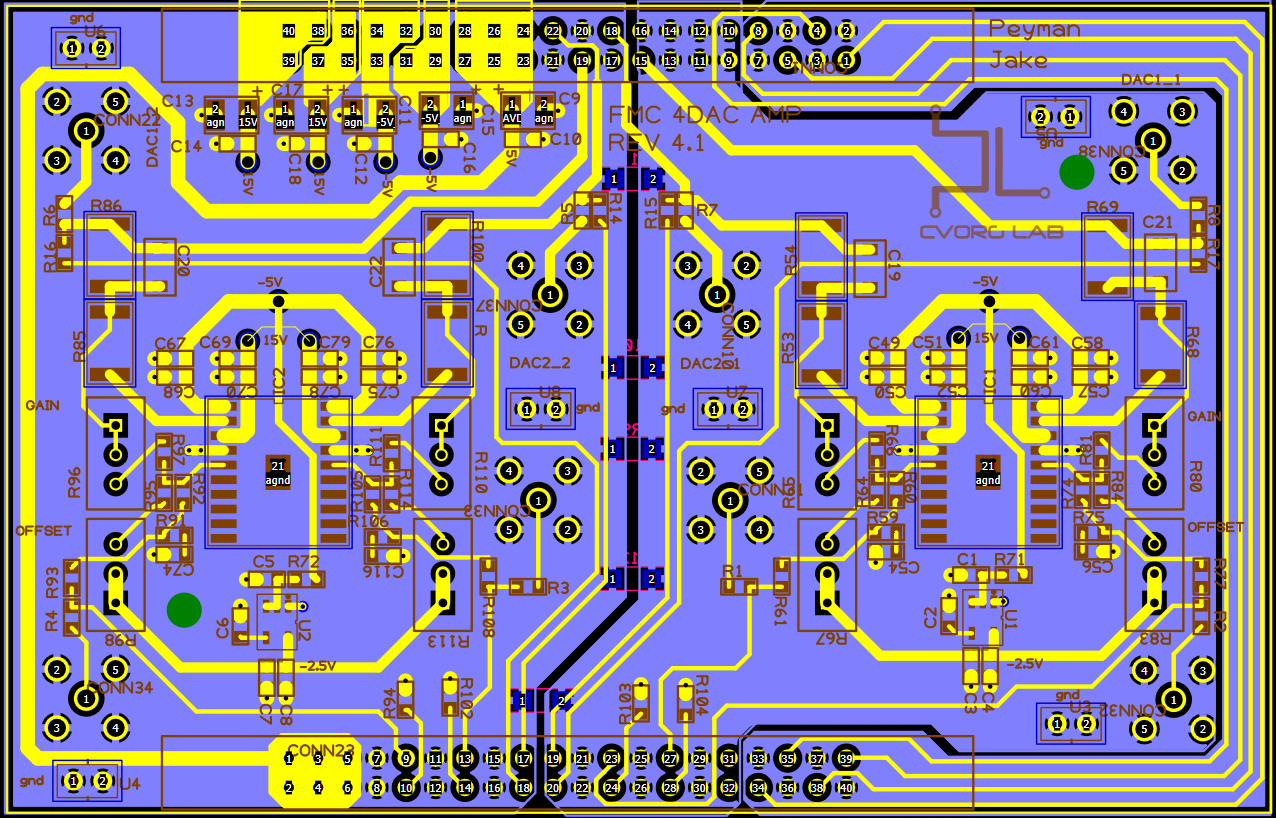
\includegraphics[width=15cm]{amp_final}
	\centering
	\caption{Final Amp Layout}
	\centering
\end{figure}

\section{Present Investigation and Review}
Unfortunately, the original designer of the amplifier circuit did not design the testing procedure  mentioned later. As such, there was no original documentation on the goals and expected outputs for the amplifier. There were multiple choices made in the PCB for theoretical future revisions that never happened. Some egregious examples include unpopulated coaxial inputs as well as a number of surface mount components. These component pads were placed with the desire to potentially investigate later. These further tests were never carried out and ended up amounting to quite a bit of wasted space on one of the system's key component boards. Due to the lack of test documentation, design methodology and stagnant development since its creation, the amp cards were targeted as a major oversight in the system's hardware that required new test procedures and a new design. Fortunately, having to use the poorly implemented test procedure allowed me to become familiar with the process and realize exactly what needed to change going forward. These new test procedures and design reviews informed the development of the second generation of amp cards.
\begin{figure}[!htb]
	\centering
	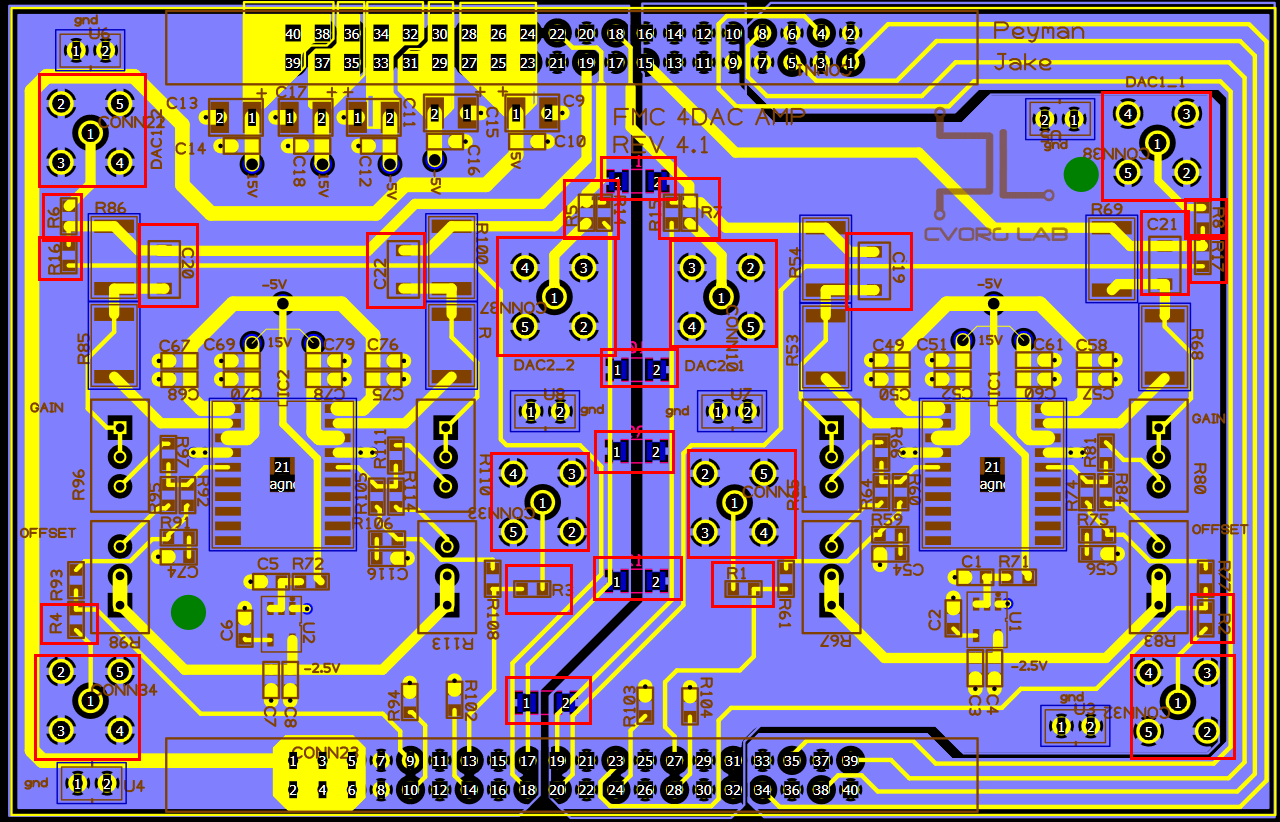
\includegraphics[width=\textwidth]{amp_empty_components}
	\caption{Unpopulated components on the amp card boxed in red. A great deal of space is wasted here}
\end{figure}
%
%Chapter 6
%
\chapter{Previous Iteration of Amplifier Testing}
The first version of the test setup and procedure was not well documented or maintained. Due to hardware changes that were too costly to warrant a complete re-fabrication, every amp card had to first be electrically reworked. The post-rework test was a simple continuity and resistance check with a multimeter to make sure all new connections were stable. Amps were then hooked up to a function generator and power supply using jumper wires from their connectors. Input and output were viewed on an oscilloscope to ensure proper amplification. While this was supposed to be a sufficient emulation of their requirements in the system, the entire procedure was loosely documented and not well-enforced enough to ensure long term reproducability and reliability.
\section{Electrical Rework}
One of the first tasks I was given upon entering the group was to help rework each amp. The first issue was that the amplifier power rails (+15V/-5V) were not connected by default. Each amplifier's power rails had to be soldered to the power output using jumper wires. This first step already provided too much room for error, as jumper wires for power distribution would not necessarily be a better choice than simply integrating power lines into the PCB. Adding a person's hand solder in between increased the risks of cold solders or accidental shorts which are completely unacceptable for power pins. \par
\begin{figure}[!htb]
	\includegraphics*[width=15cm]{amp_power_rework}
	\centering
	\caption{Rework of the power rails}
	\centering
	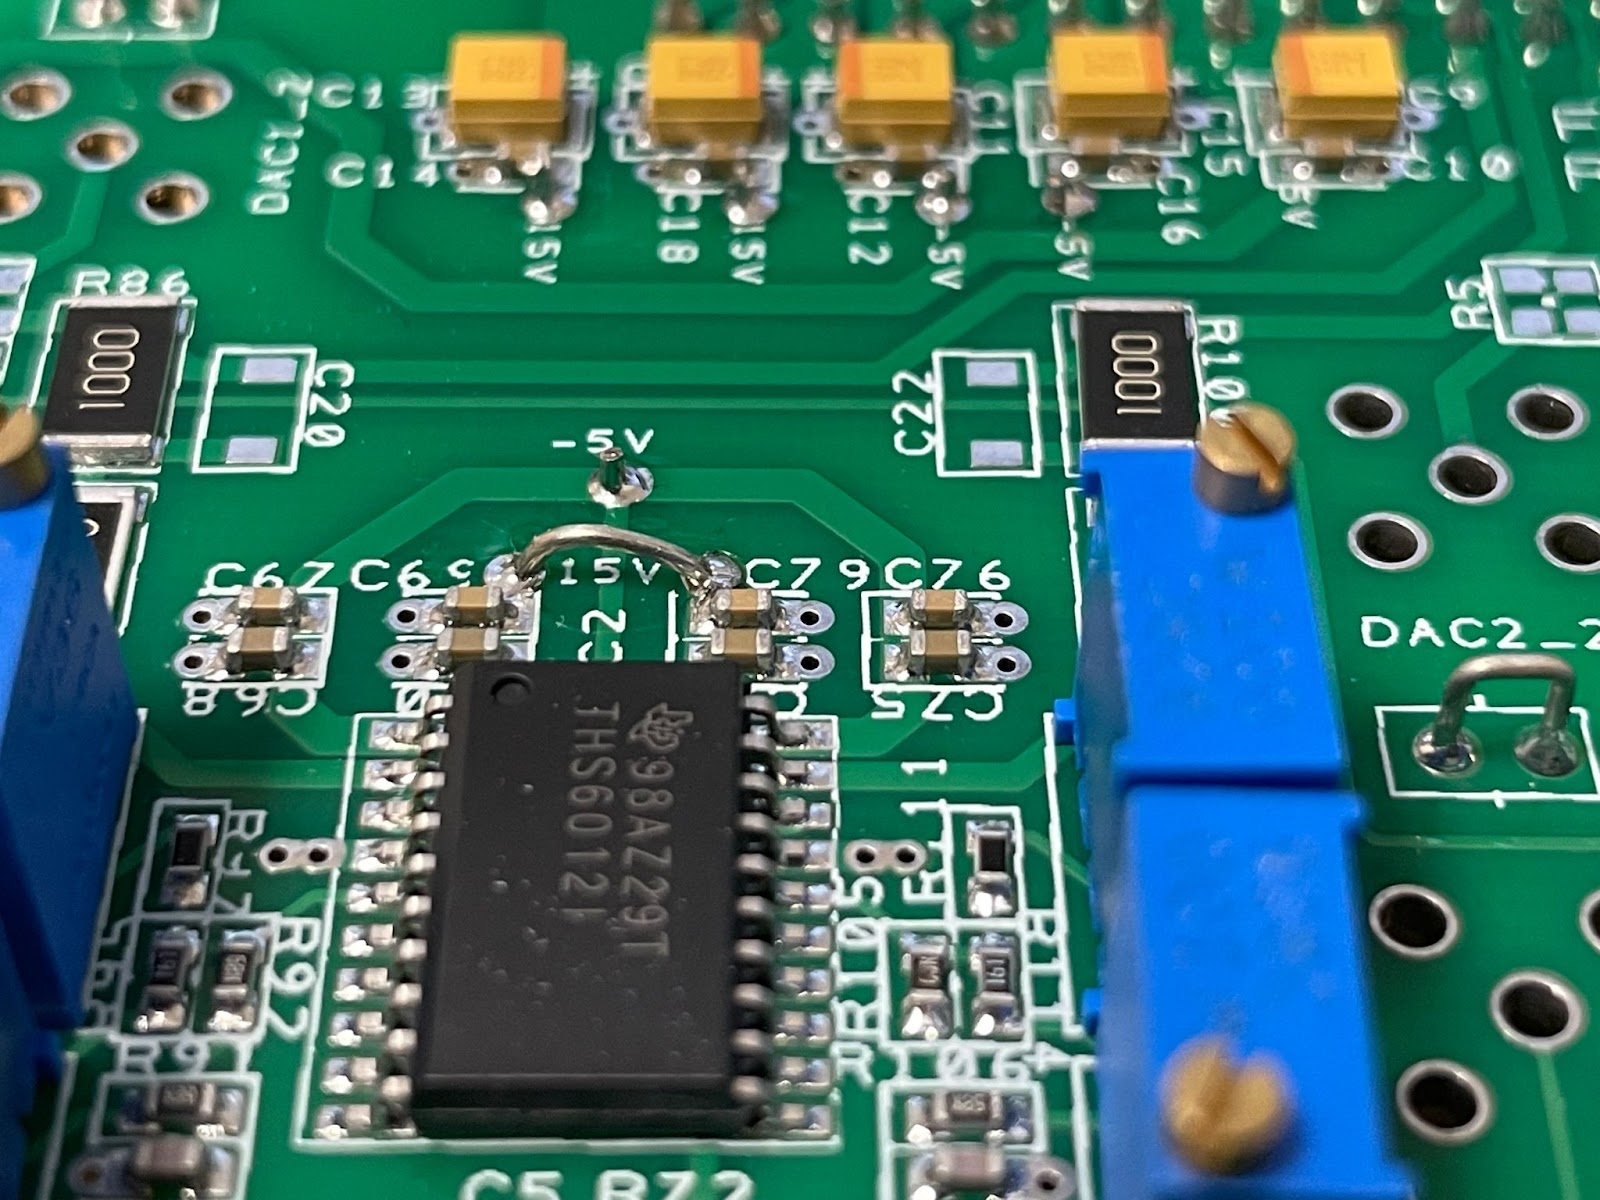
\includegraphics[width=15cm]{reworked_power_rails.jpg}
	\centering
	\caption{Power rails post-rework}
\end{figure}
\section{Component Replacement}
After bridging the power planes on the board, potentiometers and resistors had to be removed and replaced. The potentiometers were initially 100 ohms and used to control gain and offset of the amplified signals. These were replaced with 10 ohm potentiometers which was meant to allow more fine-tuned control over these values. The replaced resistors were also changed to new values to increase signal integrity. Once the rework was completed, it was to be given a brief electrical test (mentioned in the overview) to check the quality of all connections. While the continuity and resistance checks served their purpose, they were not sufficient for fully judging quality of the rework or identifying other issues early. \par
\begin{figure}[!htb]
	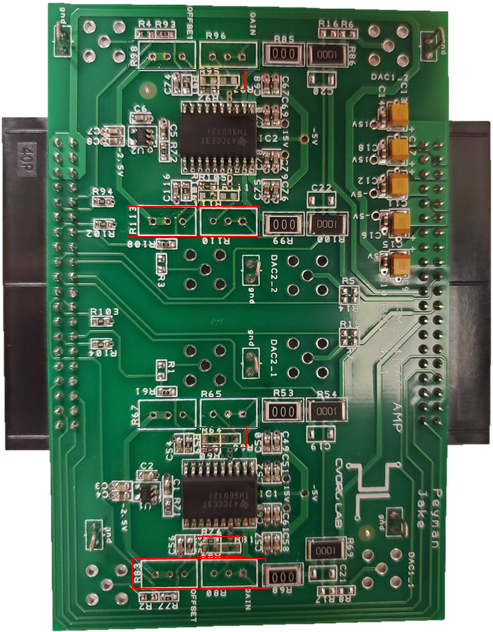
\includegraphics[width=9cm]{amp_components_rework.png}
	\centering
	\caption{Components to be removed and replaced}
	\centering
\end{figure}
The room for human error in this whole process proved to be a massive detriment. Despite a number of group members being experienced solderers, it was impossible to rework such a high volume of boards at a consistently high level of quality. The rework process introduced so many faulty cards that every post-rework card had to be ``quality checked" by a senior group member to make sure the rework was acceptable. As usual, adding another intermediary step decreased the reliability of amps and the pool of boards we had available.
\section{Electrical test}
The first stage of the electrical test consisted of the electrical checks mentioned above. There was no enforced procedure beyond following instructions on a document, and a less experienced group member ran the risk of not fully understanding what they were testing. Without detailed instructions or an intimate knowledge of the purpose of the amp, this electrical check proved to be less and less useful. \par
\begin{figure}[!htb]
	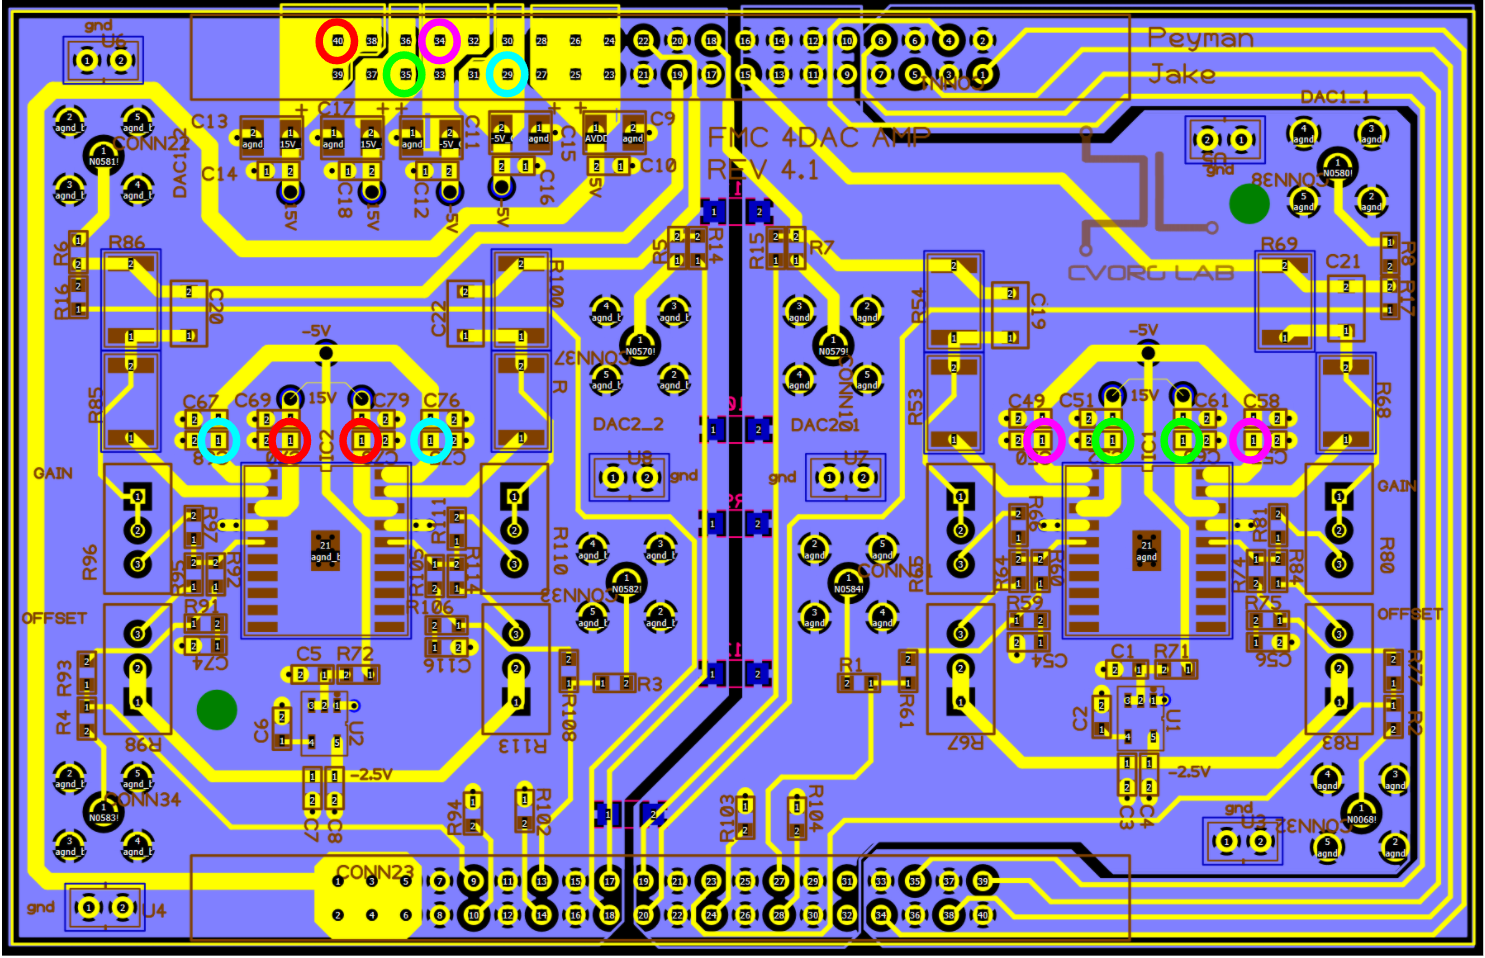
\includegraphics[width=12cm]{amp_rework_continuity.png}
	\centering
	\caption{Official documentation for the continuity checks}
	\centering
\end{figure}
\begin{figure}[!htb]
	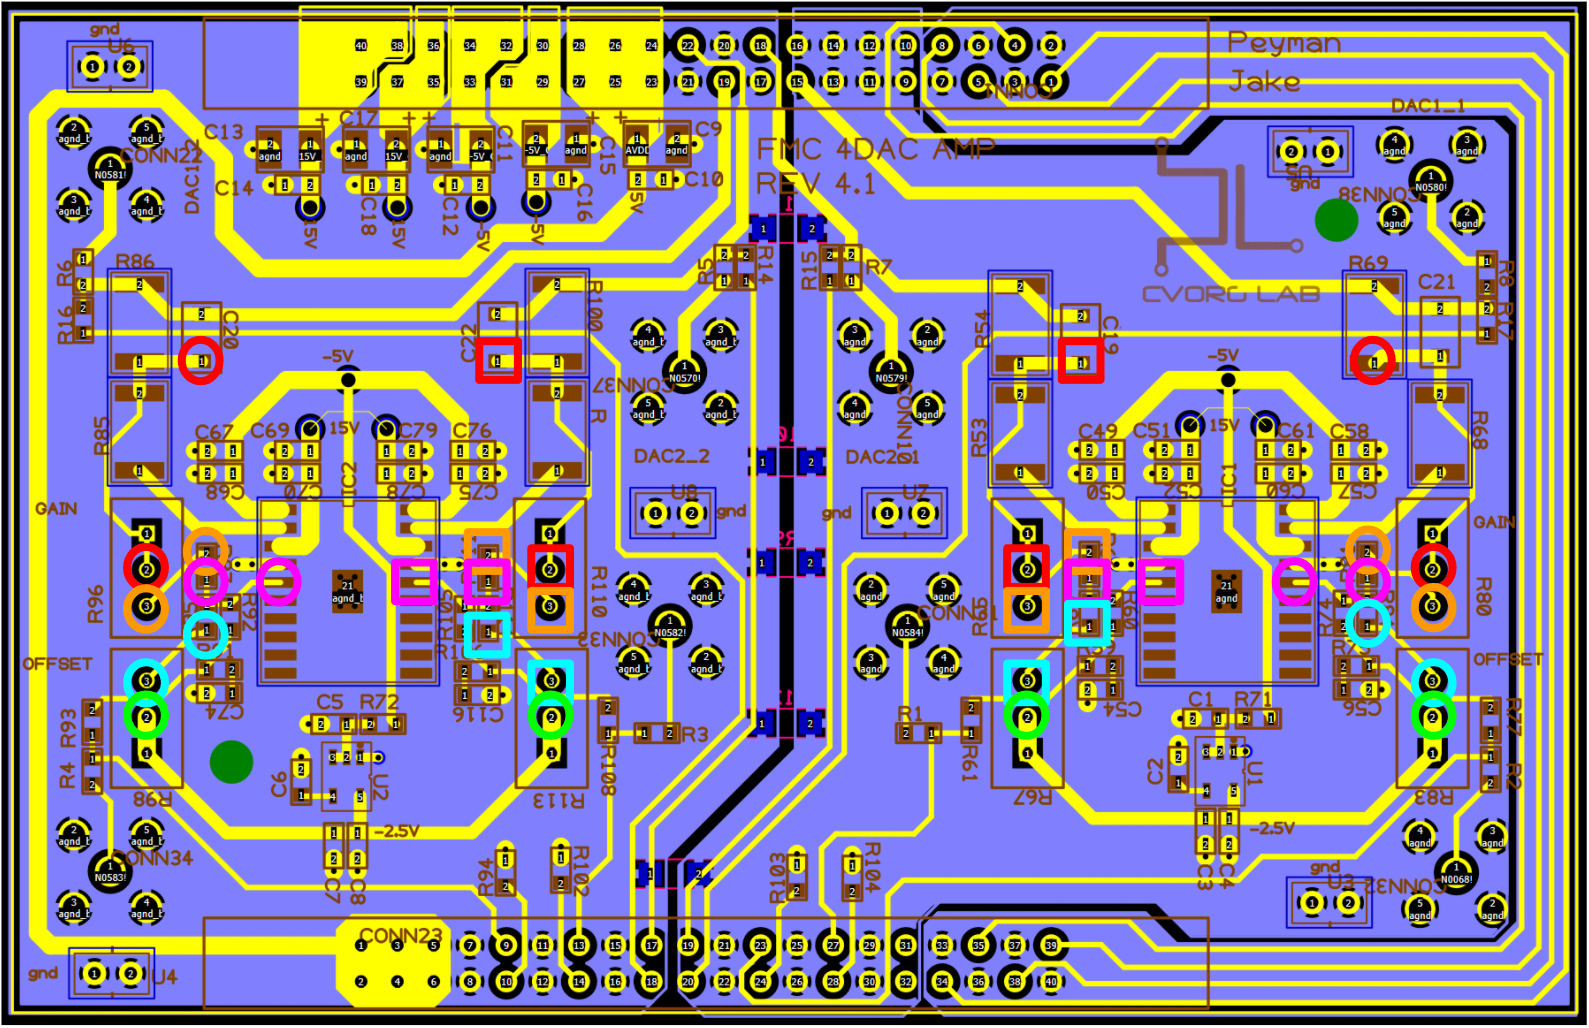
\includegraphics[width=12cm]{amp_rework_test_components.png}
	\centering
	\caption{Official documentation for checking replaced components}
	\centering
\end{figure}
The next testing stage involved hooking up instruments to simulate the type of load the amp card would have to support. This entire part of the procedure was the least well documented or understood and slowed down the validation process quite a bit. Simple breakout boards were hand-soldered for the amp connectors. Inputs were on the bottom connector and plugged into a function generator. Outputs were on the top connector and included pins for power connections (+15/-5) as well as output to the oscilloscope.
\begin{figure}[!htb]
	\centering
	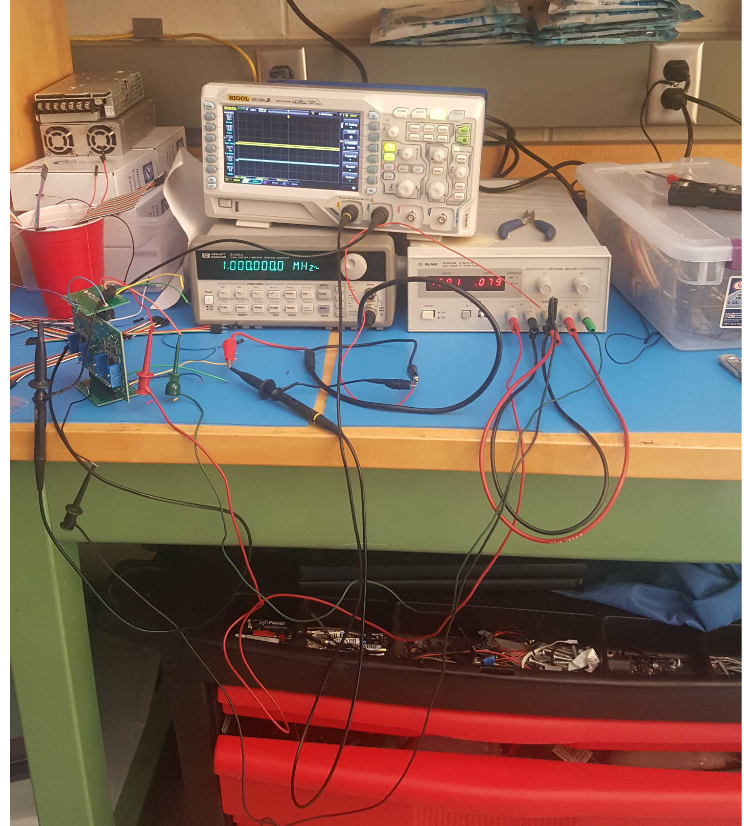
\includegraphics[width=0.5\textwidth]{amp_testing_setup}
	\caption{One of the only official pictures for a completed test setup}
\end{figure}
\subsection{Function generator}
The function generator settings used in the test were rather generic and barely modeled a realistic input for the amps in our system. Input was configured as a 1MHz square wave with an amplitude of 363mV and offset of 318mV. This function was also connected to an oscilliscope to compare against output. Using a high-speed square wave input was definitely a good idea, as a functional amplifier would output an equally square wave. Faulty components would not be able to replicate such sharp rise and settling time. The major downfall of this approach was that the function generator had to be individually tied to each of the card's four input channels, greatly increasing the amount of time a tester had to spend on moving pins and connectors. Having to manually set the wave up was also not the best idea, as this just added another area for the tester to make a mistake.
\begin{figure}[!htb]
	\centering
	\begin{subfigure}[b]{0.43\textwidth}
		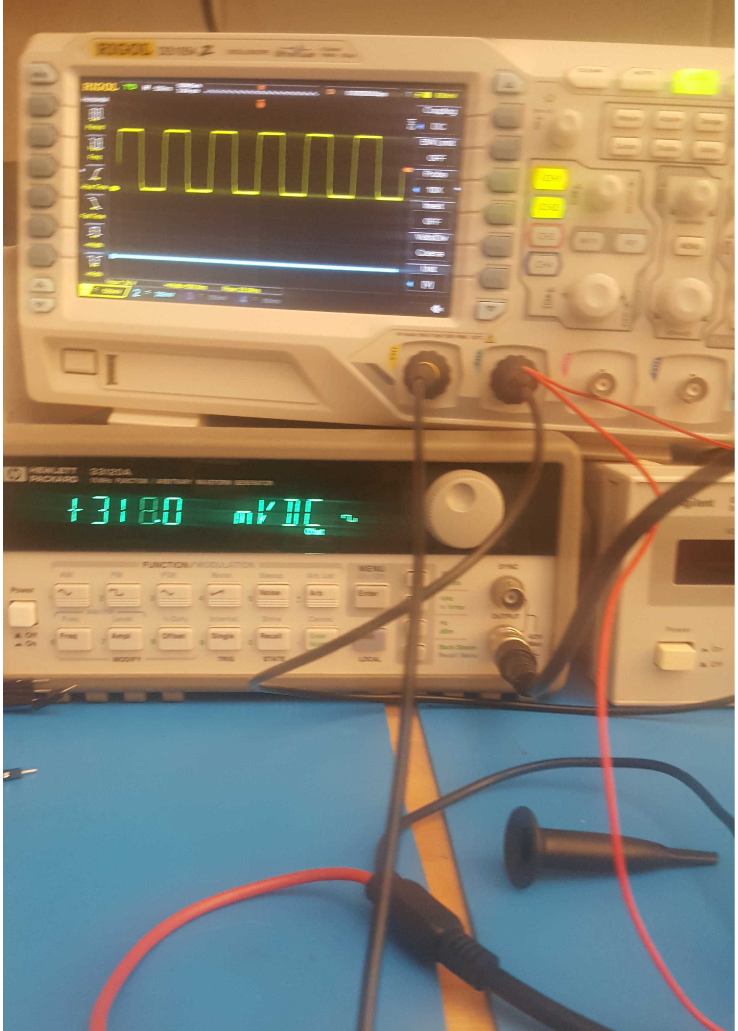
\includegraphics[width=\textwidth]{amp_functiongen_settings}
		\centering
		\caption{Function generator settings}
		\centering
	\end{subfigure}
	\hfill
	\begin{subfigure}[b]{0.5\textwidth}
		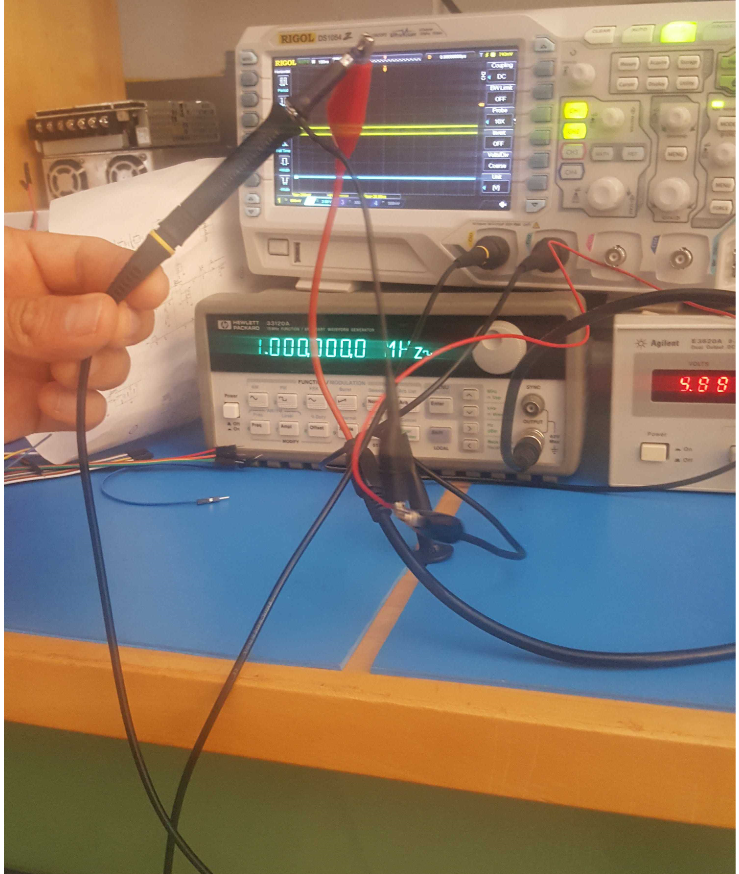
\includegraphics[width=\textwidth]{amp_functiongen_connection}
		\centering
		\caption{Function generator to scope}
		\centering
	\end{subfigure}
	\caption{Offical documentation for setting up the function generator. Insufficient to teach anybody new how to use the equipment.}
\end{figure}
\subsection{Power supply}
Setting up the power rails was a little bit less involved. The user only needed to attach +15V, -5V, and GND to the top breakout board. Connections were still made using extruding jumper wires and alligator clips, yet another point of concern when testing a large number of amps. There were hardly any examples of what a correct setup would look like in the testing document at this point.
\begin{figure}[!htb]
	\centering
	\includegraphics*[width=0.8\textwidth]{amp_powersupply}
	\caption{Official reference image for the amp power supply}
\end{figure}
\subsection{Measuring Output}
As mentioned before, output would be measured on an oscilloscope. Amplitude of input and output could be easily compared by human eyes and the next channel would be connected. This was a slow process that involved manyally re-attaching input and output alligator clips. If gain or offset needed to be tweaked, the tester was to turn their respective potentiometers and observe output. The move to 10 ohm potentiometers greatly decreased their effect on the circuit at all and ended up being more of a nuisance than a useful control signal.
\begin{figure}[!htb]
	\centering
	\includegraphics*[width=0.5\textwidth]{amp_scope_output}
	\caption{Official example of oscilloscope output. Yellow=input, blue=output}
\end{figure}
\section{Lessons Learned}
In conclusion, learning and using the amplifier rework and test procedures was a difficult task that left far too much room for interpretation or error. The amplifiers were crucial to the system's integrity but were not thoroughly tested or maintained. The process was slow, tedious and quite disconnected from the functionality of the system. Poor documentation meant that only a few group members truly understood the purpose and functionality of all steps involved. Swapping cards under test required disconnecting the card from its breakout boards that were already precariously grasped by alligator and probe clips from the instruments. The breakout board pins were not even labled, so it was difficult to determine if issues were due to the user or hardware. This procedure may have filled its need when first conceived, but proved to be unsustainable as the project scaled up. A careful re-examination was required to understand what needed to be tested and what could be improved.

%
% Chapter 7
%
\chapter{Development of a Formal Testing Procedure}
\section{Initial considerations}
The new procedure was desgined as a direct response to the previous one. Based on complaints and difficulties from all who had to use the setup, we compiled a list of the biggest concerns and focused the procedure design around them. These included:
\begin{itemize}
	\item Manually changing input/output channels was slow and introduced too many steps
	\item Input \& output were connected through a flimsy probe clip
	\item No way to separate amp power rails
	\item No indication if the amps were receiving sufficient power
	\item No data collection for comparison between cards
	\item No standards or documentation for gain/offset potentiometer tweaks
\end{itemize}
\section{Design Choices}
The first readily apparent issue lay in the fact that there was a great deal of manual setup being performed by testers which was not ideal for long-term or large-scale testing. Amp cards were delivered in relatively small batches and had to be reworked and tested as they came. Having to search for a procedure that was hard to understand was not a good solution. I opted to use Python drivers communicating over the two serial specifications (USB serial and VX11 over Ethernet) to automate the input generation and output measurement. By having direct software access to the wave being generated and the data collection, users were in control of a closed loop from beginning to end. The remainder of the issues remained in the lack of hardware support for testing. Input and output locations were unclear and pin placement was only known to those who created the boards, unless testers wanted to open the PCB files and check themselves. By designing a pair of new PCBs to solve this issue, the test station had a clear set of instructions and devices to measure and capture data as was needed.

\section{Software Control}
Controlling the instruments available in our lab took a bit of research. While other group members had used some of the automation tools before, this was one of the first fully scripted hardware test setups in the lab. The communication protocols and code libraries required are explored below.
\subsection{pySerial Overview}
PySerial is a simple Python library to build and push serial commands over a variety of protocols. This library allows programmers to script serial access and build their own commands to be used for any device they require. For this application, I needed to build commands for a function generator. Other members of the group had previously automated this device and were able to provide documentation on the serial commands necessary. The benefit of a simple serial protocol was that it required no proprietary software and could be modified or extended for other devices. Initiating communication with a serial device is simple with pySerial as the programmer can simply can all serial ports and view device properties. In this specific application the serial device was the only one connected to the host computer, which allowed the device detection to be quite straightforward:\par
\begin{lstlisting}
	ports = list(serial.tools.list_ports.comports())
	for port, desc, hwid in sorted(ports):
		print("{}: {} [{}]".format(port, desc, hwid))
	for p in ports:
		print("USB Serial: {}".format(p.description))
		if "USB-SERIAL" in p.description:
				print("Found the FeelTech AWG")
				awg = feeltech_awg.FeelTechAWG(p[0])
	assert awg is not None, "No AWG device found"
\end{lstlisting}
To understand the process of communicating with this device I traced example commands to their lowest levels. To command the device to do anything, requests first had to be packaged into a recognizable prefix. To generate a prefix, parameters must be packaged in a particular order: \par
\begin{lstlisting}
	assert rw in range(2), "R/W value for prefix must be 0 (read) or 1 (write)"
	prefix_rw = "W" if rw == 1 else "R"
	assert channel in (1, 2), "Invalid channel, must be set to 1 (main) or 2 (auxilary)."
	prefix_channel = "M" if channel == 1 else "F"
	valid_modifiers = ("W", "F", "A", "O", "D", "P", "N")
	assert modifier in valid_modifiers, "Invalid cmd modifier (%s), must be in %s"%(modifier, valid_modifiers)
	return prefix_rw + prefix_channel + modifier
\end{lstlisting}
This command prefix is then concatenated with a desired parameter based on the function being controlled. Turning on an output channel, for example, takes in an output flag and attaches it to the command prefix:
\begin{lstlisting}
	"""
	output:  int -> 0 to turn channel off, 1 to turn channel on
	"""
	cmd = _generate_cmd_prefix(1, channel, "N") + str(output)
\end{lstlisting}
The command is now ready to be sent to the device. Using pySerial functions for read/write operations, the code is simple:
\begin{lstlisting}
	self.device.flushInput()
	self.device.write((cmd_str + "\n").encode())
	self.device.flush()
\end{lstlisting}
The straightforward nature of serial communications made this easy to debug and test. The function generator only needed to perform a few tasks (turn channels on/off, set waveform parameters) the scope of my research into its functionality was limited. I believe, however, that this establishes a good base for future testing development. Many other instruments use specifications such as VISA which may be a better choice in the future.
\FloatBarrier
\subsection{VXI11 Overview}
The VXI11 Communication Protocol is an architecture based on the VMEbus architecture meant for electronic communication. VXI11 in particular was built as an instrument communication spec \cite{vxi}. VXI11 requires three channels and operates over Ethernet.\par
VXI11 Python libraries are available and make VXI communication simple. Similarly to serial, commands must be constructed by the programmer and packaged into strings sent over the VXI bus. For example, writing to the device makes a device-level system call to write the input data to a predetermined location. From the programmer's point of view, one only has to use the high-level functions to facilitate communication. There are, for example, functions for read(), write(), and ask(), which performs a write and then read. These functions are grouped and abstracted for use with this specific instrument. If, for example, the programmer wants to ask the device what a selected channel's probe ratio is, the code is as follows:
\begin{lstlisting}
	def get_probe_ratio(self, channel):
		"""
		Returns the probe ratio for a specific channel
		"""
		channel = self._interpret_channel(channel)
		return float(self.query(':{0}:PROBe?'.format(channel)))
\end{lstlisting}
The string being pushed in the query function is a device-specific string that is outlined by the manufacturer \cite{rigol}. Using the listed commands and an ethernet connection, the VXI11 bus will automatically detect when a valid device is connected to the local network through Ethernet. The IP address of the device is specified upon initialization and needs to be checked before running tests.

\section{Input Stage}
The input stage of the amp testing procedure was the first to be targeted. Directing input to the amp card should be a simple task for the user. Since all four channels are used in parallel on the system, they can be connected to a unified signal source and displayed together on the oscilloscope for data collection. Using a mix of hardware and software support I developed an input procedure for the new test.
\subsection{Function Generation}
To implement a Python layer for the function generator I opted to use a FeelTech FY6900 Arbitrary Waveform Generator.
\begin{figure}[!htb]
	\centering
	\includegraphics*[]{awg}
	\caption{FeelTech FY6900}
\end{figure}
This was a relatively cheap function generator that fulfilled the tasks we needed to accomplish. With up to 60MHz sine wave output, this device was more than enough to test the capabilities of the amplifiers. The DAC input the amps were designed to process were at frequencies far below this. For the first versions of the test I opted to use the original function generator settings until more could be determined about the input parameters. The code was simple and based on the previously listed libraries \& protocols:
\begin{lstlisting}
	awg.set_on_off(1, 0)
	awg.set_on_off(2, 0)

	awg.set_waveform(1, 1)
	awg.set_frequency(1, 1000000)
	awg.set_amplitude(1, x[i])
	awg.set_offset(1, 0.318)
	awg.set_phase(1, 0)

	# Turn channel 1 on
	awg.set_on_off(1, 1)
\end{lstlisting}
For the automated test to save time, it was set to loop four times to collect plot data from the oscilloscope for all four amplifier output channels. In order for this automatic switching to work, hardware had to be designed to accept the signal and distribute it accordingly.
\subsection{Bottom (Input) PCB}
Major flaws in the original test setup included the lack of any shielded cable to transfer the input signal and the tester having to manually clip the input to each amp channel. Although we were not necessarily testing for strict signal integrity, it is better practice to use standard connectors for input rather than probe clips. Since the FeelTech generator used a BNC connector it was easiest to match this on the input card. BNC connectors are shielded coaxial connectors capable of reliably passing signals under 4GHz and less than 500V \cite{bncbook}. \par
Separating the amplifier's input lines was a useless step that only served to complicate the process. To solve this I had to examine the amp's PCB layout to find the relevant pins. The DAC inputs were differential pairs identified within the layout below:
\begin{figure}[!htb]
	\centering
	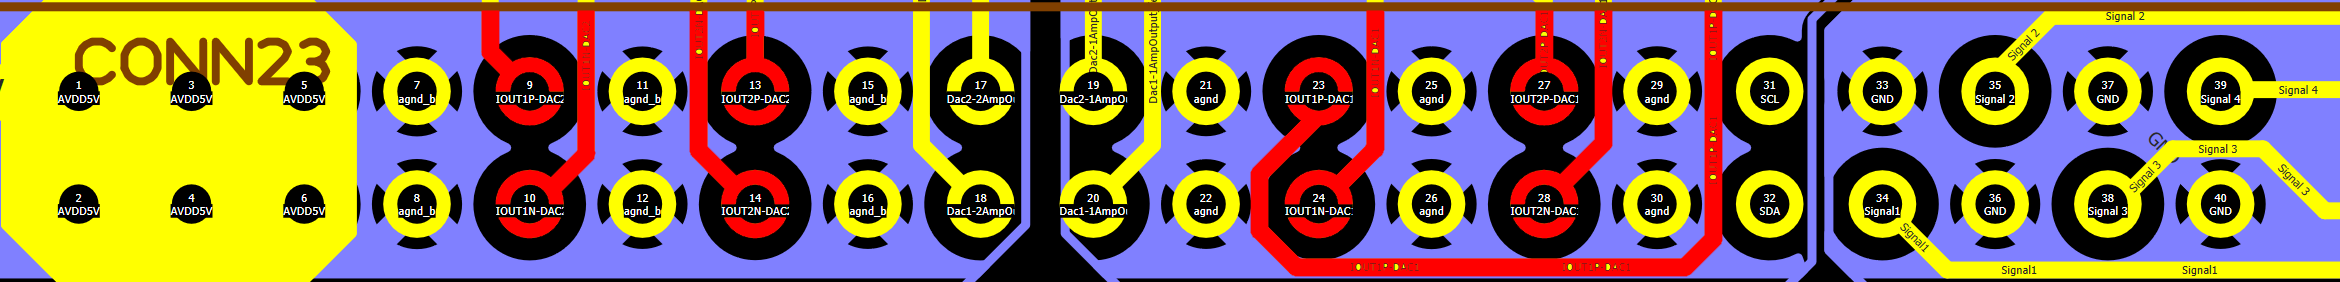
\includegraphics[width=\textwidth]{amp_input_pins}
	\caption{Differential input pins on the Amp PCB}
\end{figure}
The input side of the board was fairly simple to draw and lay out. One of the amp's purposes was to turn the DAC's differential output into a single-ended output. To accomplish this, the amp card terminated the N-terminals of all incoming DAC signals through a 49 ohm resistor.
\begin{figure}[!htb]
	\centering
	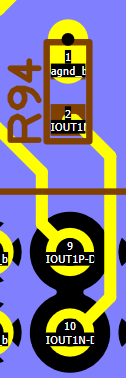
\includegraphics{amp_n_p}
	\caption{Terminating resistor for the N-terminal of the DAC output.}
\end{figure}
Grounding the differential input was an acceptable decision for the test setup. Only the P-lines of the signal would be processed by the circuit at all, so they were routed together and joined to a single BNC input in the test board.
The layout followed shortly and included a ground plane to maximize signal integrity. With such a limited number of relevant pins on the input side of the amp card, designing the test board was not an issue. \par
\subsection{Input Conclusion}
This section of the test setup resulted in a far simpler procedure. Having to only connect one output through a stable connection and clearly labeled board eliminated all possible confusion for testers. INSERT PICTURE OF BOARD HERE
\begin{figure}[!htb]
	\centering
	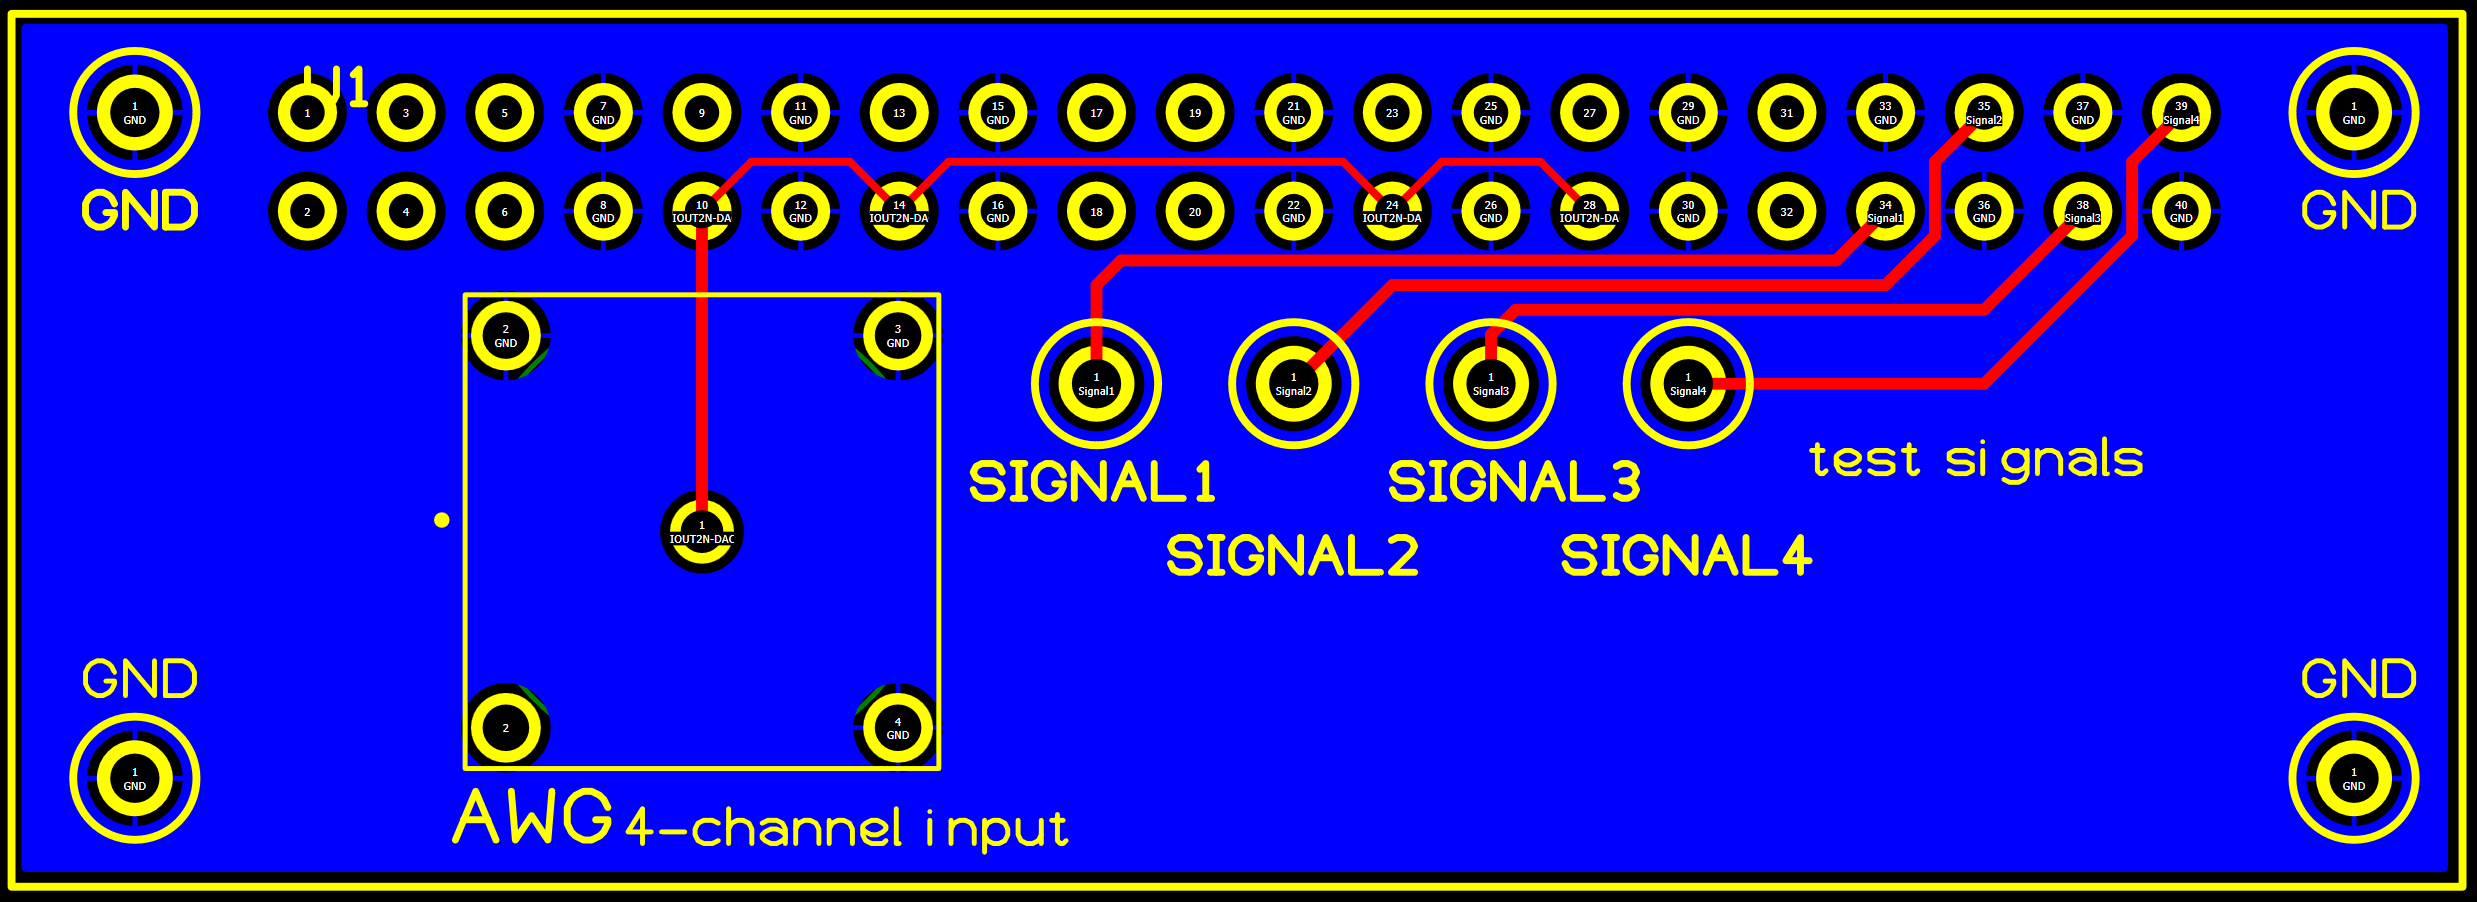
\includegraphics[width=\textwidth]{amp_bottom_layout.png}
	\caption{Input Test board layout}
\end{figure}
\begin{figure}[!htb]
	\centering
	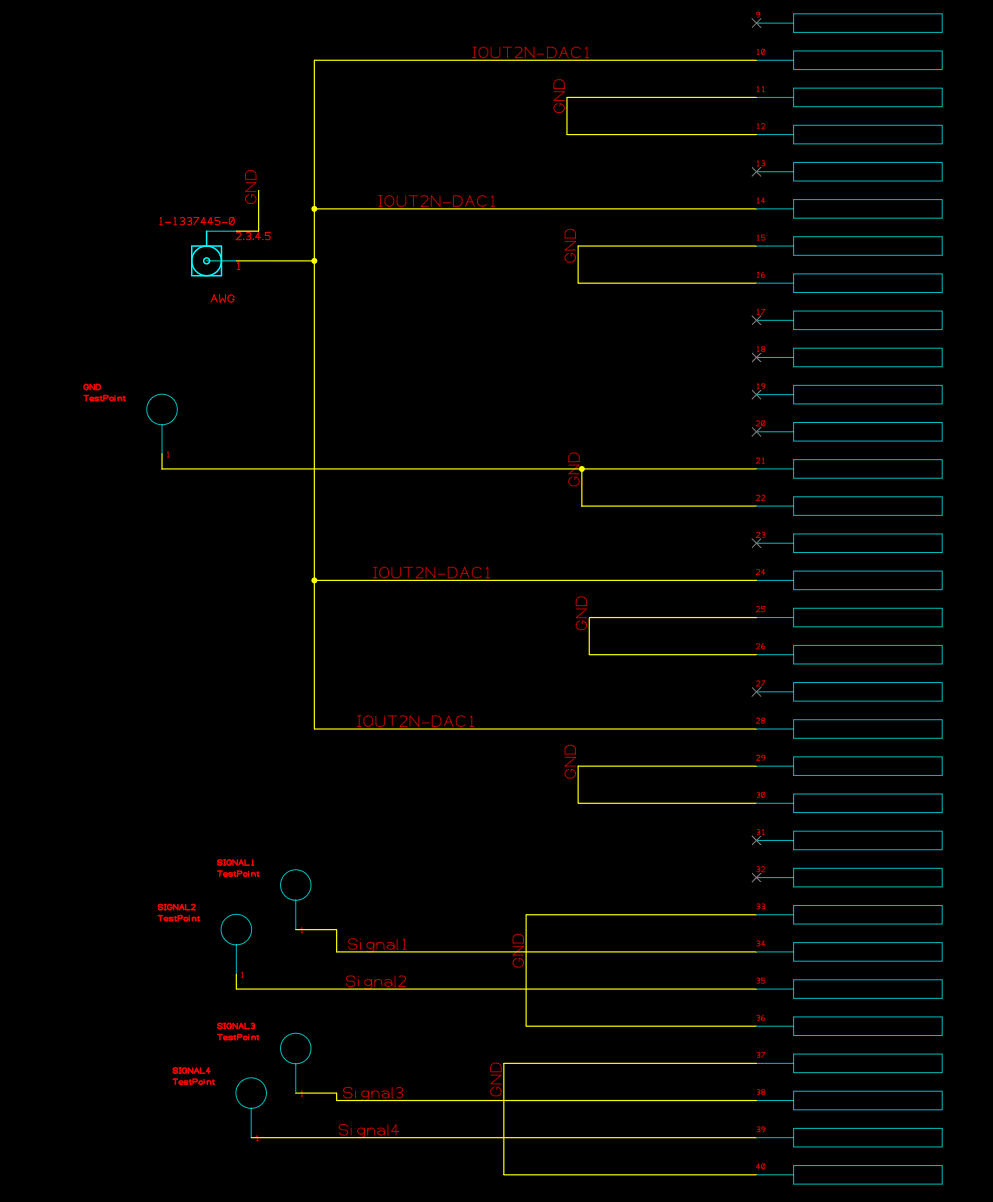
\includegraphics[width=\textwidth]{amp_bottom_schematic.png}
	\caption{Input Test board schematic for joining P-inputs and grounding N-inputs}
\end{figure}

\section{Output Stage}
The output of the amp card required the testers to be able to view all output channels at once as well as collect and plot the oscilloscope's data. This once again required a mix of software and hardware tools to accomplish.
\subsection{Top (Output) PCB}
Before any data could be routed to the oscilloscope we needed to develop a control system for the top connector of the amp card. This connector housed a number of vital pins including power rail input and amplifier output. In the system, this connector would be attached to the interface board and transport signals through the ribbon cables. To appropriately test the functionality of all amp cards, users had to be able to fulfill a number of requirements:
\begin{itemize}
	\item Ensure power was being properly delivered to both amplifiers
	\item Have the ability to independently toggle power to each amplifier unit
	\item Route output through shielded cable to oscilloscope
\end{itemize}
Each section of the PCB was therefore designed to address these issues. To indicate valid power delivery a simple LED indicator system was sufficient. Each amplifier had its own pin for power delivery and as such could be routed independently. A switch with three positions was used to control power delivery. When in neutral, power would be routed to both amplifiers A and B. When flipped left or right, the switch would direct power into only amplifier A or B respectively. The LED indicators were placed into voltage dividers. If enough voltage was being delivered on that line, the divider would pass voltage to light up the LED. \par
When moving on to the layout the main concern was for space and signal integrity. By keeping the board as symmetrical as possible and including another ground plane, the design was ensured to be safe from interference. The four output channels were available as BNC headers as well and could be directly connected to a 4-channel oscilloscope. The switch and LED components provided the most challenges in layout as they required quite a few traces. The final layout was compact and clearly labeled to show testers what they needed to use. Power delivery was accomplished through probe clips to the power supply. The power supply is never changed or adjusted during the whole process, so the clips were not any issue when detatching and reattaching cards from the testing boards.
\begin{figure}[!htb]
	\centering
	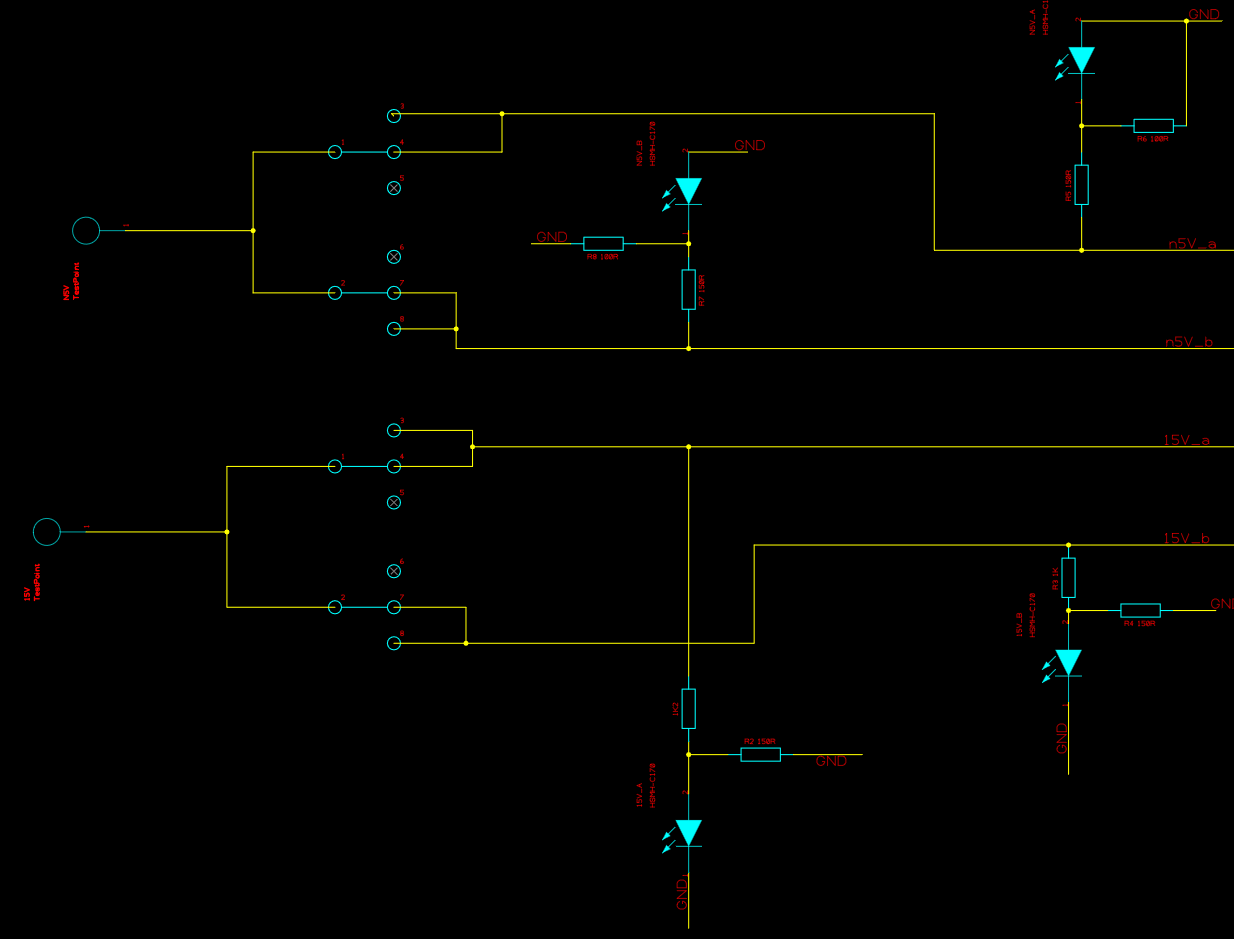
\includegraphics[width=\textwidth]{amp_top_power_indicators.png}
	\caption{Power indicator \& switching circuits for the -5V and +15V lines}
\end{figure}
\begin{figure}[!htb]
	\centering
	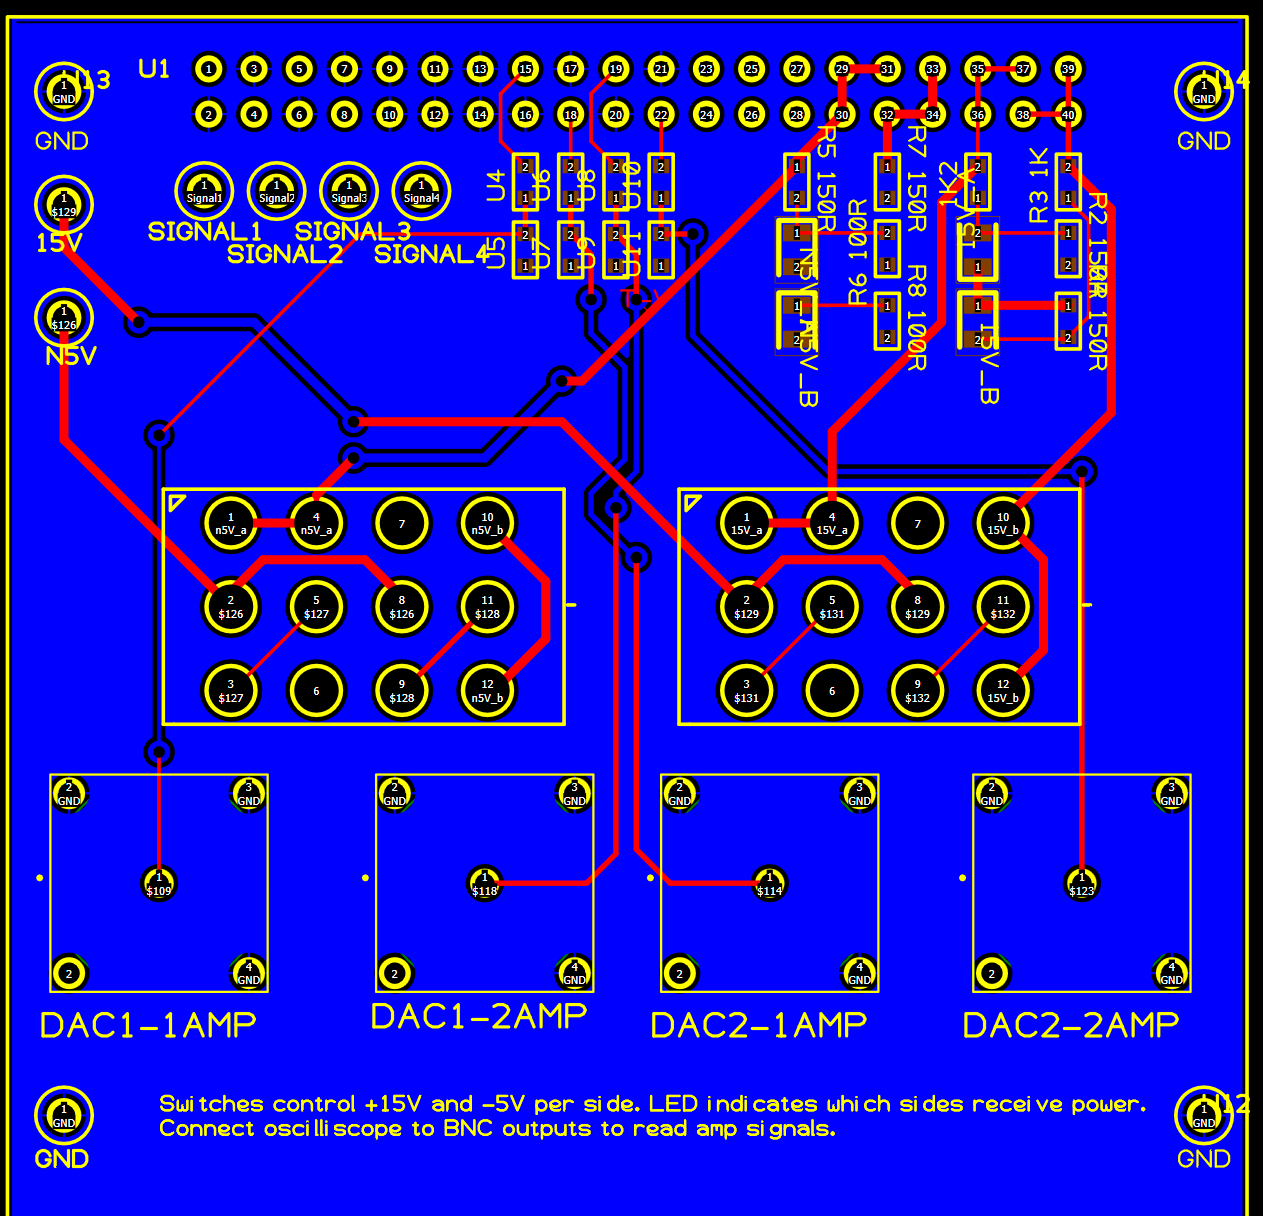
\includegraphics[width=\textwidth]{amp_top_layout}
	\caption{Finished layout of Top testing board}
\end{figure}

% %
% This is the References file (ref.tex)
%
\renewcommand{\bibname}{References}
\begin{thereferences}
Lastname, Firstname  ``Title.''  \textit{Journal}, Year.

Lastname, Firstname, and Firstname Lastname.  \textit{Title of Book}.  Publisher, Year.
\end{thereferences}
      % This file (ref.tex) contains the text
                   % for the references.
                   
%%
% This is the Bibliography file (bib.tex)
%
% For 100-999 change 99 to 999; for 1000-9999 change 99 to 9999 
\begin{thebibliography}{99}
\bibitem{1}Lastname, Firstname  ``Title.''  \textit{Journal}, Year.

\bibitem{2}Lastname, Firstname, and Firstname Lastname.  \textit{Title of Book}.  Publisher, Year.
\end{thebibliography}
      % This file (bib.tex) contains the text
                   % for a bibliography.
                                      
%%
% This is the Bibliography file (bibtex.tex)
% This generally works for BibTeX

% Use sample.bib for BibTeX database
\bibliography{sample}
% BibTeX style (plain, alpha, unsrt)
\bibliographystyle{plain}
	 % This file (bibtex.tex) contains the text
                   % for a bibliography if using BibTeX with
                   % sample.bib
                                      
%%
% This is one Appendix file (app.tex)
%
\oneappendix{Title for Appendix}

This is the information for one appendix. This is to be used if there is only one appendix.      % This file (app.tex) contains the text
                   % for one Appendix. 
                   
\bibliography{refs} % Entries are in the refs.bib file

\bibliographystyle{plain} % We choose the "plain" reference style

%
% This is the Appendix A file (appA.tex)
%
\appendix{Title of Appendix}

This is the information for the first appendix, Appendix A. Copy the base file, appA.tex, for each additional appendix needed such as appB.tex, appC.tex, etc. Modify the main base file to include each additional appendix file.

If there is only one appendix, then modify the main file to only use app.tex instead of appA.tex.     % This file (appA.tex) contains the text
                   % for Appendix A. 
                   
\include{appB}     % This file (appB.tex) contains the text
                   % for Appendix B.   
       

\end{document}